\begin{figure}[t]
\centering
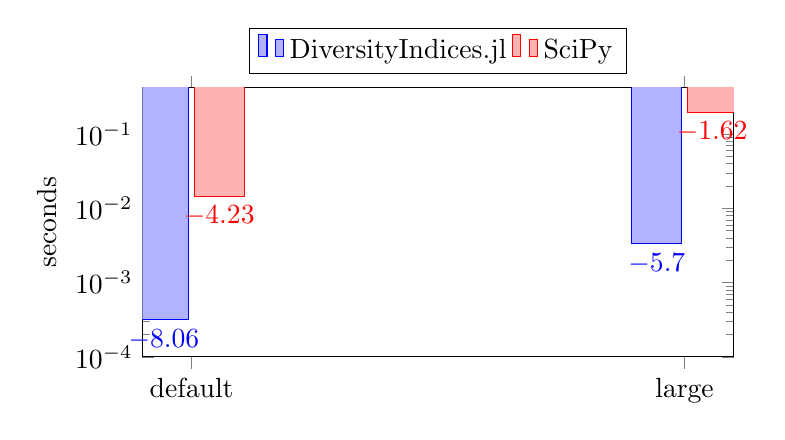
\begin{tikzpicture}
\begin{axis}[
  ybar,
  bar width=18pt,
  ymode=log,
  ylabel={seconds},
  symbolic x coords={default,large},
  xtick=data,
  legend style={at={(0.5,1.05)},anchor=south,legend columns=2},
  width=0.75\linewidth,
  height=5cm,
  ymin=0.0001,
  nodes near coords,
  nodes near coords align={vertical},
]
\addplot coordinates {(default,0.000315) (large,0.00336)};
\addplot coordinates {(default,0.0145) (large,0.197)};
\legend{DiversityIndices.jl,SciPy}
\end{axis}
\end{tikzpicture}
\caption{Selected Jaccard distance matrix timings after bitset incidence encoding. The benchmark is workflow-level and hardware-dependent, but illustrates the algorithmic benefit of packed incidence representation.}
\label{fig:jaccard}
\end{figure}
